
\section{Appendix}\label{sec:appendix}


\subsection{Activation function}
\noindent The function $\Phi_{\cdot}$ is defined by combining a generalized version of the sigmoid, namely with a gain $\beta \neq 1$ and offset $\alpha\neq 0$, and a Gaussian with mean $\mu$ and variance $\sigma$. Their contributions are weighted by as $r$ and $1-r$ ($r\in(0,1)$) respectively.

\begin{equation*}
    \Phi_v(x) = r\left(1 + \exp^{-\beta(x-\alpha)}\right)^{-1} + (1-r)\exp\left(-\frac{(x-\mu)^2}{2\sigma^2}\right)
\end{equation*}

\noindent The motivation behind this choice is to express a function that possesses a bounded region (depending on $\mu,\,\sigma$) at a high/low peak (depeding on the value of $\gamma_{2}$), and a continuous transition to a constant value (depending on the steepness of the sigmoid $\beta$, shift
$\alpha$, and intensity $\gamma_{1}$).

\begin{figure}[H]
    \centering
    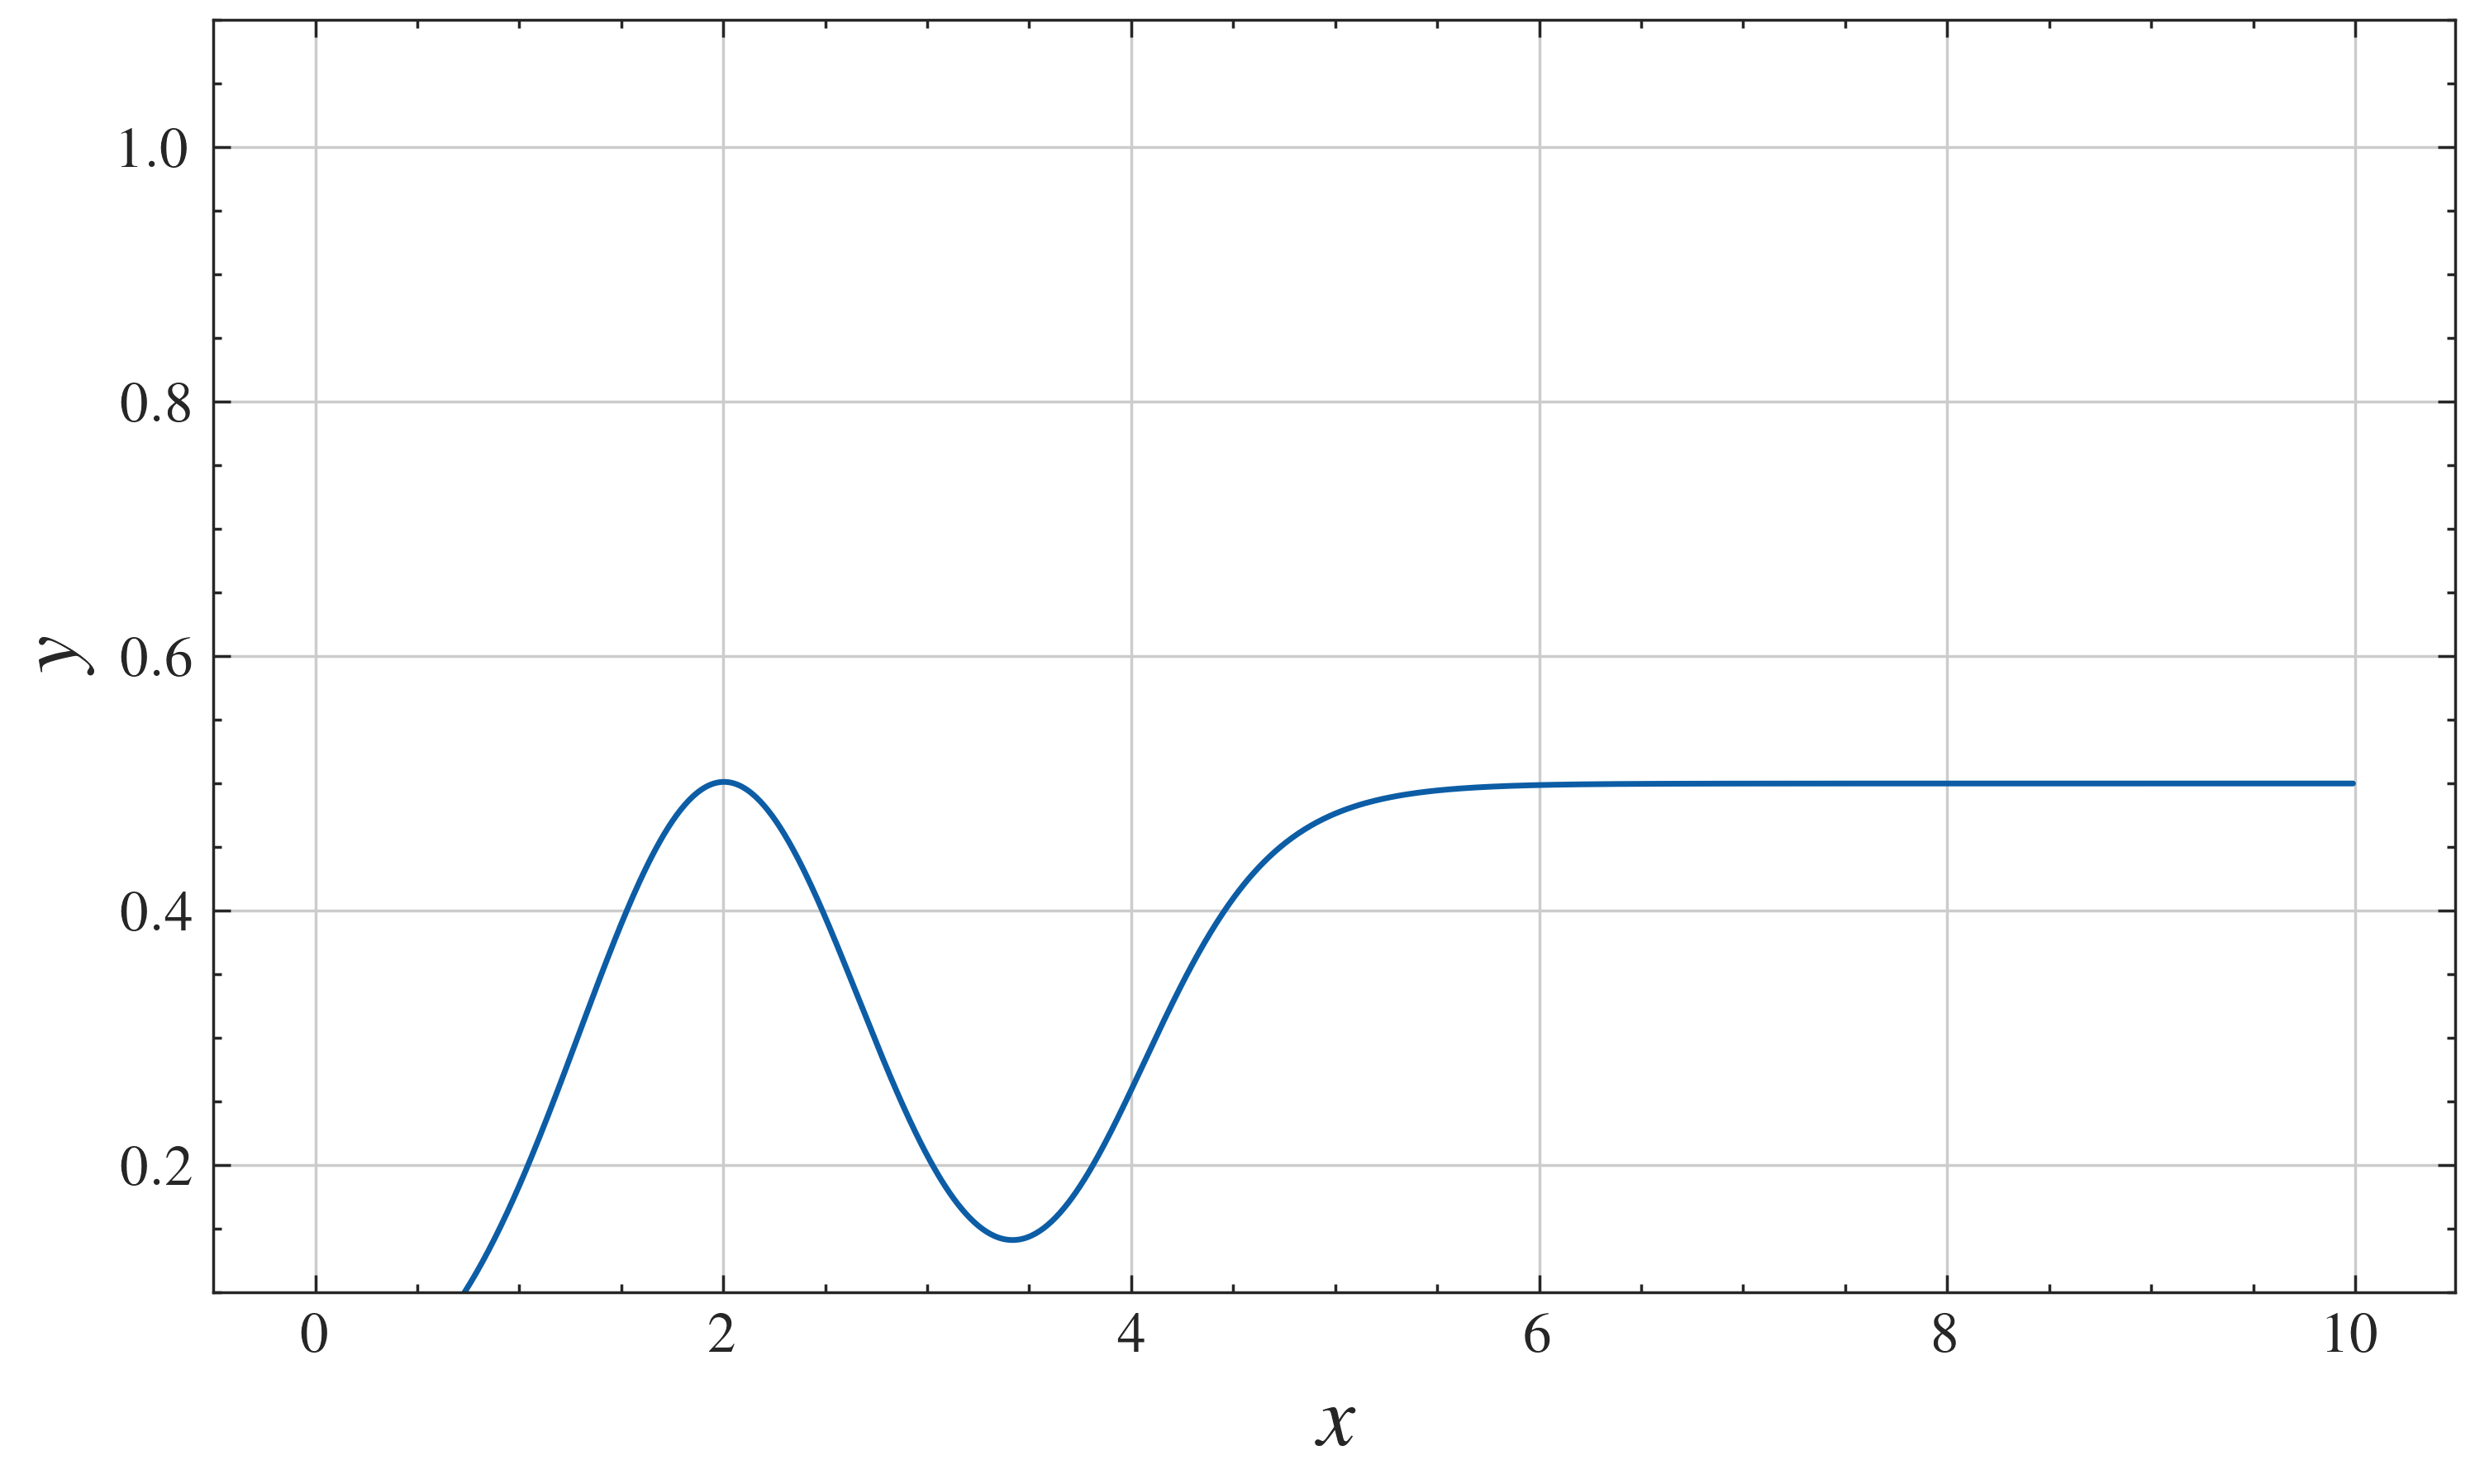
\includegraphics[width=0.8\textwidth]{figures/gaussian_sigmoid.png}
    \caption{\textsc{Activation function $\Phi_{v}$} - \textit{Parameters $\beta=10$, $\alpha=1$, $\mu=1$, $\sigma=1$, and $r=0.5$.}}
    \label{fig:gau_sigm}
\end{figure}

\newpage
